\documentclass[titlepage=false,12pt]{scrreprt}

\usepackage[utf8]{inputenc}
\usepackage[T1]{fontenc}
\usepackage{lmodern}
\usepackage[ngerman]{babel}
\usepackage{amsmath}
\usepackage[backend=bibtex]{biblatex}
\usepackage{tikz}
\usepackage{amsthm}
\usepackage{amssymb}
\usepackage{xcolor}
\usepackage{framed}
\usepackage{tabto}
\usepackage{capt-of}
\usepackage{pgfplots} % loads tikz
\pgfplotsset{compat=1.7}
\usepackage{csquotes}
\usepgfplotslibrary{fillbetween}
\usetikzlibrary{intersections}
\usepackage{graphicx}
\graphicspath{{./../img/}}

\pgfdeclarelayer{bg}
\pgfsetlayers{bg,main}

\colorlet{shadecolor}{gray!15}

\usepackage{hyperref}
\hypersetup{
	colorlinks,
	citecolor=black,
	filecolor=black,
	linkcolor=black,
	urlcolor=black
}

\newtheorem{definition}{Definition}[chapter]
\AfterEndEnvironment{definition}{\noindent\ignorespaces}

\newcommand{\listingsettings}{%
	\lstset{%
		language=C++,			% Standardsprache des Quellcodes
		%numbers=left,			% Zeilennummern links
		%stepnumber=1,			% Jede Zeile nummerieren.
		%numbersep=5pt,			% 5pt Abstand zum Quellcode
		%numberstyle=\tiny,		% Zeichengrösse 'tiny' für die Nummern.
		breaklines=true,		% Zeilen umbrechen wenn notwendig.
		breakautoindent=true,	% Nach dem Zeilenumbruch Zeile einrücken.
		postbreak=\space,		% Bei Leerzeichen umbrechen.
		tabsize=2,				% Tabulatorgrösse 2
		basicstyle=\ttfamily\footnotesize, % Nichtproportionale Schrift, klein für den Quellcode
		showspaces=false,		% Leerzeichen nicht anzeigen.
		showstringspaces=false,	% Leerzeichen auch in Strings ('') nicht anzeigen.
		extendedchars=true,		% Alle Zeichen vom Latin1 Zeichensatz anzeigen.
		captionpos=b,			% sets the caption-position to bottom
		%backgroundcolor=\color{ListingBackground}, % Hintergrundfarbe des Quellcodes setzen.
		xleftmargin=0pt,		% Rand links
		xrightmargin=0pt,		% Rand rechts
		frame=single,			% Rahmen an
		frameround=ffff,
		rulecolor=\color{darkgray},	% Rahmenfarbe
		%fillcolor=\color{ListingBackground},
		keywordstyle=\color[rgb]{0.133,0.133,0.6},
		commentstyle=\color[rgb]{0.133,0.545,0.133},
		stringstyle=\color[rgb]{0.627,0.126,0.941},
		aboveskip=1.5em,
	}
}

\clubpenalty = 10000 % schließt Schusterjungen aus (Seitenumbruch nach der ersten Zeile eines neuen Absatzes)
\widowpenalty = 10000 % schließt Hurenkinder aus (die letzte Zeile eines Absatzes steht auf einer neuen Seite)
\displaywidowpenalty=10000

\bibliography{bibliography}

\title{MVVM: Model-View-ViewModel}
\subtitle{Advanced Softwareengineering - DHBW Stuttgart}
\author{Nico Vogel, Lukas Sopora}
\date{31.12.2019}

\begin{document}
\maketitle
	
{\renewcommand\clearpage\relax
	\tableofcontents}
\newpage

\chapter{Einleitung zu MVVM}

\section{Anwendungsbereiche von MVVM}

Bereits vor der Veröffentlichung von MVVM wurden bei der Entwicklung von Applikationen mit einer grafischen Benutzeroberfläche Design Patterns angewandt, 
mit denen der Programmcode sinnvoll in Komponenten eingeteilt werden konnte, mit dem Ziel, den Überblick und die Wartbarkeit der Applikation für den Entwickler zu vereinfachen.
\\\\
\noindent
Das bekannteste dieser Patterns, welches auch heute noch häufige Verwendung findet, ist das Model-View-Controller (MVC) Pattern.
Aus diesem entwickelte sich auch das Model-View-Presenter (MVP) Pattern, woraus 2004 wiederum das Presentation-Model (PM) hervorging.
2005 wurde schließlich vom Microsoft Architekten John Gossmann das Model-View-ViewModel (MVVM) Pattern als Spezialisierung des Presentation Model vorgestellt.
Seitdem wird es vor allem in C\# im Zusammmenhang mit WPF, aber auch in Delphi, Silverlight und AngularJS angewandt.
\\\\
\noindent
Alle oben erwähnten Patterns verfolgen denselben Ansatz, den Programmcode sinnvoll aufzuteilen und die Oberflächenbeschreibung der Benutzeroberfläche von der Programmlogik zu trennen. \par

\section{Was ist das Problem das MVVM angeht?}

Das MVVM Pattern geht Probleme der klassichen UI Programmierung an und bringt zudem einige Vorteile mit sich:
\\\\
\\noindent
In erster Linie nimmt das Pattern das Problem an, dass UI und Logik stark voneinander abhängig sind, wenn keine klare Trennung vorgenommen wird.
Dadurch wird die Wartbarkeit des Programmcodes erheblich beschwert,  

ANMERKUNG: Das ist nur reinkopiert und muss noch umgeschrieben werden @Lukas

Wird in der UI Entwicklung eingesetzt und soll folgende Probleme angehen:
	
\begin{itemize}
	\item Starke Abhängigkeit zwischen UI und Logik
	\item Redesign problematisch
	\item Cross Platform
	\item schwer zu testen
\end{itemize}

\subparagraph{Vorwort}


MVVM wird bei der Entwicklung von Applikationen mit UI angewandt.
Dabei werden einige Probleme angegangen:
Generell kommt es auf die Ausgangessituation an, wie stark die folgenden punkte gewogen werden.

\begin{itemize}
	\item UI und Logik ist ein code, was schwer zu warten ist 
	\item da die UI und die logik viel miteinander zu tun haben kann man nicht einfach das design ändern. dabei zerstört      man wahrscheinlich viele funktionen usw.
	      Auch ist eine Abstraktion der View in vielen Fällen nicht möglich
	\item Zudem gibt es Frameworks, wie CrossMVVM, die die Anwendung des Patterns auf Cross Platform ermöglichen
	\item Außerdem kann man durch die Trennung von UI und Logik die Logik automatisiert testen
\end{itemize}
\subparagraph{Schlusswort}
wenn beispielweise Application Layer angewandt wird, ist punkt 1 schonmal deutlich weniger schlimm, da man bereits eine saubere trennung zwsichen UI und Logik hat.

\chapter{Wie ist MVVM aufgebaut?}

MVVM besteht aus mehreren Komponenten die ineinandergreifen. Die drei 
größten sind Model, View und ViewModel. Dabei wir das Zusammenspiel 
der Komponenten in der Abbildung X dargestellt. Die View und das ViewModel 
können Bidirektional kommunizieren, während das ViewModel nur das Model
aufruft beziehungsweise verwendet.

ABBILDUNG X

\section{Komponenten}

\paragraph{Model}

Das Model umfasst nur Daten und maximal noch Logik für die Daten. 
Im C\# Umfeld spricht man auch von POCO (Plain old Control Object) 
oder in Java POJO (Plain old Java Object).
	
Das folgende Beispiel beschreibt eine Schülerklasse die der Definition 
eines Models entspricht.

CODE BEISPIEL SCHÜLER

\paragraph{ViewModel}

Mithilfe des ViewModels werden Informationen und Funktionen zusammengefasst
in eine Klasse, damit eine View diese verwenden kann. Das ViewModel verwenden zur 
Informationsbereitstellung die Models. Die bereitgestellten Funktionen sind
entweder in dem ViewModel selbst oder in separaten Klassen implementiert.

\paragraph{View}

Die View ist ausschließlich zur Darstellung der Inhalte und bereitstellen der
Funktionen über Schaltflächen oder ähnliches gedacht. Dabei wird in der View
Binding verwendet um Inhalte und Funktionen von dem ViewModel zu verwenden.

\section{Kommunikation}

Nachdem nun die Hauptkomponenten beschrieben sind, fehlt noch wie diese miteinander 
kommunizieren. Hierbei werden Models zwischen der View und dem ViewModel ausgetauscht.
Dieser Austausch wird über Binding, Events und Commands realisiert.

\paragraph{Binding}

Binding gibt es grundsätzlich in zwei Variationen. Diese sind in Abbildung 2.1 dargestellt. OneWay Binding
lässt Kommunikation nur in eine Richtung zu, somit von dem ViewModel zur View und umgekehrt.
Letzteres nennt man in C\# auch OneWayToSource. Die zweite Variante ist TwoWay Binding ermöglicht
der View als auch dem ViewModel Informationen an den jeweils anderen zu senden. Zusätzlich ist 
bei WPF das OneTime Binding vertreten, wobei die Zieleigenschaft nur beim Start der Applikation 
oder, wenn sich die DataContext Eigenschaft ändert, also wenn der View Komponente ein neues 
ViewModel zugewiesen wird.

\begin{figure}[h]
	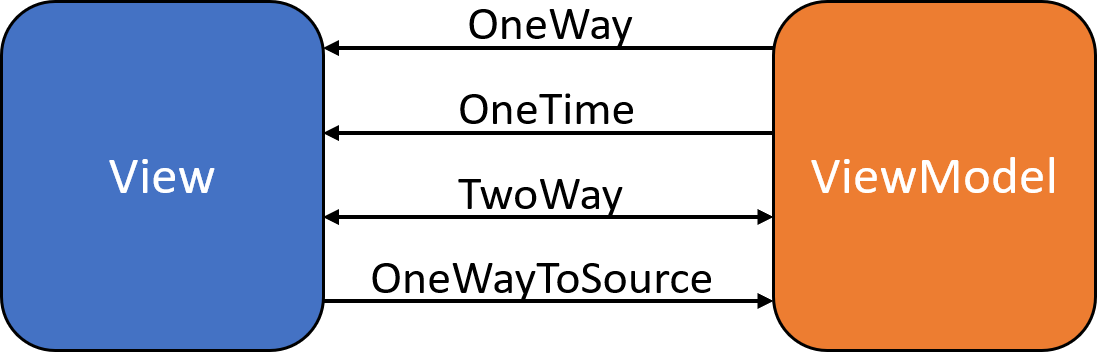
\includegraphics[width=\textwidth]{Wpf_Binding.png}
	\caption[]{DataBinding}
\end{figure}


\paragraph{Event}

Events sind Ereignisse von UI Komponenten auf die andere Komponenten sich registrieren 
können um so zusätzlichen Code auszuführen. Es gibt eine breite Menge an Events die
von Komponenten zur Verfügung gestellt wird. Diese können wiederum nicht mit Binding 
kombiniert werden und daher ist es notwendig in C\# in der Code-Behind Datei
die verlinkung zum ViewModel herzustellen.

\paragraph{Command}

Commands sind Events die über Binding verwendet werden können. Hierbei ist eine schlecht
abdeckung gegeben, weshalb häufig auf Events zurückgegriffen werden muss. Ein Command
beinhält auch keine Informationen, sonder ist nur ein Trigger einer Methode. Ein Beispiel
ist Button klick.

\section{Wo ordnet sich MVVM in Application Layer ein?}

Da in Anwendung in der Regel auch mit Strukturpattern realisiert wird, wird in der Abbildung X
das MVVM Pattern in das Application Layer Model eingefügt. Hierbei ist wichtig, dass das
ViewModel sowohl in der Presentation, als auch in der Business Layer vertreten ist. Das kommt
daher, dass das ViewModel einerseits Methoden und Properties für die View aggregiert und andererseits
Business Code ausführt.  

ABBILDUNG X - Application layered

\chapter{Beispiel des MVVM Patterns in C\# WPF}

Das MVVM Pattern kommt aus C\# Windows Presentation Foundation (WPF) Applicationen, daher
wird in dem folgenden Abschnitt ein Beispiel in C\# WPF zur Veranschaulichung von MVVM gezeigt.


@Lukas: das darfst du schreiben

\chapter{Verglich zwischen MVVM und MVC}

In diesem Abschnitt wird beschrieben wie sich MVVM zu MCV (Model View Controller) unterscheidet. 
Zu beginn wird das MVC Pattern erläutert um daraufhin die Unterschiede hervorzuheben. 

\paragraph{Was ist MVC?}

Das Model View Controller Pattern ist erstmals im Kontext der Programmiersprache SMART verwendet 
worden. In diesem Fall sind Komponenten, wie Eingabefelder, mit dem MVC Pattern realisiert worden.
Mit dem aufkommen von Komplexeren Sprachen ist auch der Scope von MVC gewachsen. Bei TODO(passende Sprache/Framework eingesetzen)
entspricht die View einer Komponente oder Seite.

Jede der drei Bestandteile von MVC hat seine eigene Aufgabe. Das Verhältnis unter den Komponenten
ist in Abbildung X dargestellt. Die View ist für die Darstellung und
Animation zuständig. Das Model stellt die Daten zur Verfügung, die in der View dargestellt werden.
Der Controller verbindet View und Model, da diese sich nicht kennen. Somit steht der Controller 
über der View und dem Model, wodurch Model und View entkoppelt sind, aber darfür eine starke Bindung
zum Controller besteht. 

ABBILDUNG X - MVC

\paragraph{Vergleich der beiden Pattern}

Während bei dem MVC Pattern der Controller das Verbinden der Komponenten übernimmt, wird das
in dem MVVM Pattern über Binding realisiert und ein externes System löst das Binding am ende auf.
Bei MVC kennt die View das Model nicht, aber bei MVVM ist der View das ViewModel bekannt.
Das wird auch in der Abbildung X dargestellt durch die Verbindungen der Komponenten.

TODO vielleicht noch bissel mehr dazu sagen

ABBILDUNG X - MVC vs MVVM

\chapter{Kritische betrachtung des MVVM Patterns}



Pro

<span class="text-left">

- flexibel
- steile Lernkurve (OOP, Testing, Binding)
- gut testbar

</span>
</div>

<div class="rdiv">

Con

<span class="text-left">

- viel code für wenig resultat
- XAML Notation umfangreich
- Binding undurchsichtig

</span>

\end{document}